% copyright (c) 2018 Groupoid Infinity

\documentclass{article}
\usepackage[english,russian]{babel}
\usepackage{listings}
\usepackage{amsmath}
\usepackage{amssymb}
\usepackage{amsthm}
\usepackage{mathtools}
\usepackage{url}
\usepackage{tikz-cd}
\usepackage[utf8]{inputenc}

\theoremstyle{definition}
\newtheorem{theorem}{Теорема}
\newtheorem{definition}{Визначення}
\newtheorem{exercise}{Вправа}
\newtheorem{example}{Приклад}
\newcommand*{\incmap}{\hookrightarrow}
\newcommand*{\thead}[1]{\multicolumn{1}{c}{\bfseries #1}}
\lstset{basicstyle=\small,inputencoding=utf8}

\addto\captionsrussian{\renewcommand{\contentsname}{Зміст}}
\addto\captionsrussian{\renewcommand{\bibname}{Список використаних джерел}}
\addto\captionsrussian{\renewcommand{\abstractname}{Аннотація}}


\begin{document}

\title{Мови програмування \\ для квантових обчислень}
\author{Максим Сохацький $^1$}
\date{ \small $^1$ Національний технічний університет України \\
       «Київський Політехнічний Інститут» ім. Ігора Сікорського \\
       28 жовтня 2018 }
\maketitle

\begin{abstract}
Ця робота є спробою огляду існуючих мов програмування
для квантових обчислень та їх особливостей.
\\
{\bf Ключові слова}: Теорія типів, Мови порграмування, Квантові обчислення
\end{abstract}
\tableofcontents

\newpage

\section{Попередні відомості}

\subsection{Лінійна алгебра}

Нотація Дірака це компактний формалізм лінійної алгебри який будемо застосовувати
для визначень квантової механіки.

\begin{table}[h]
\centering
  \caption{Нотація Дірака}
 \begin{tabular}{lll}
    \hline
       Нотація & Визначення \\
    \hline
       $|\psi\rangle$ & загальний кет-вектор, наприклад $(c_0,...,c_n)^T$ \\
       $\langle\psi|$ & дуальний бра-вектор, наприклад $(c_0^*,...,c_n^*)$ \\
       $|n\rangle$    & n-й базис вектор стандартного базису $N=(|0\rangle,...,|n\rangle)$\\
       $|\tilde{n}\rangle$    & n-й базис вектор альтернативного базису $\tilde{N}=(|\tilde{0}\rangle,...,|\tilde{n}\rangle)$ \\
       $\langle\phi|\psi\rangle$ & скалярний добуток \\
       $|\phi\rangle\otimes|\psi\rangle$ & тензорний добуток \\
    \hline
  \end{tabular}
\end{table}

\begin{definition} (Векторний простір). Множина V називається векторни мпростором над
скалярним полем F, тоді і тільки тоді, коли визначені операції $+ :V \times V \rightarrow V$ (сума векторів)
та $\cdot:F\times V\rightarrow V$ (добуток скаляра та вектора) з наступними властивостями:
i) $(V,+)$ утворюють комутативну групу;
ii) $\lambda |\psi\rangle = |\psi\rangle \lambda$;
iii) $\lambda(\mu|\psi\rangle) = (\lambda\mu)|\psi\rangle$;
iv) $(\lambda+\mu)|\psi\rangle = \lambda|\psi\rangle + \mu|\psi\rangle$;
v) $\lambda(|\psi\rangle+|\varphi\rangle) = \lambda|\psi\rangle + \lambda|\varphi\rangle$.
Далі будемо розглядати скалярне поле комплексних чисел $F=C$.
\end{definition}

\begin{definition} (Скалярний добуток).
Функція $\langle\cdot|\cdot\rangle:V\times V\rightarrow C$ називається скалярним
добутком, тоді і тільки тоді, коли:
i) $\langle\psi|(\lambda\varphi\rangle+\mu|\chi\rangle) = \lambda\langle\psi|\varphi\rangle+\mu\langle\psi|\varphi\rangle$;
ii) $\langle\psi|\varphi\rangle = \langle\varphi|\psi\rangle^*$;
iii) $0 < \langle\psi|\psi\rangle \in \mathbb{R}$.
Скалярний добуток визначає норму
$\parallel|\psi\rangle\parallel = \sqrt{\langle\psi|\psi\rangle} = \parallel\psi\parallel$.
\end{definition}

\begin{definition} (Повний векторний простір).
Нехай V векторний простір з нормою $\parallel\cdot\parallel$ та $|\psi_n\rangle \in V$
послідовність векторів.
i) $|\psi\rangle$ є послідовністю Коші ттт. $\forall\epsilon>0\exists N>0 : \forall n,m> N, \parallel |\psi_n\rangle - |\psi_{n+1}\rangle\parallel < \epsilon$.
ii) $|\psi\rangle$ сходиться ттт. $\forall\epsilon>0\exists N>0 : \forall n> N, \parallel |\psi_n\rangle - |\psi\rangle\parallel < \epsilon$.
Простір V повний ттт. кожна послідовність Коші сходиться.
\end{definition}

\begin{definition} (Гільбертів простір).
Повний векторний простір H зі скалярний добутком $\langle\cdot|\cdot\rangle$ та
відповідною нормою $\parallel\psi\parallel=\sqrt{\langle\psi|\psi\rangle}$ називається Гільбертовим.
\end{definition}

\begin{definition} (Лінійний оператор).
Нехай V -- векторний простір, а А -- функція $A : V \rightarrow V$. Тоді А
називається лінійним оператором ттт.
$$
A(\lambda|\psi\rangle + \mu|\varphi\rangle) = \lambda A |\psi\rangle + \mu A |\varphi\rangle
$$
В $C^n$ лінійний оператор є матрицею $m \times n$
з елементами $a_{i,j} = \langle i | A | j \rangle$, де $A = \Sigma_{i,j} a_{i,j} | i\rangle\langle j|$.
За визначенням лінійності оператор А можно записати через лінійну суму векторів базису B:
$$
A : |n\rangle \rightarrow \Sigma_k a_{kn}|k\rangle, \text{\ де\ } |k\rangle \in B.
$$
\end{definition}

\begin{definition} (Тензорний добуток гільбертових просторів).
Нехай $H_1$ та $H_2$ --- Гільбертові простори з базисами $B_1$ та $B_2$.
Тоді тензорний добуток
$$
H = H_1 \otimes H_2 = \{ \Sigma_{|i\rangle \in B_1} \Sigma{|j\rangle \in B_2} c_{ij}|i,j\rangle \| c_{ij} \in \mathbb{C} \}.
$$
також Гільбертів простір з базисом $B = B_1 \times B_2$ та скалярним добутком:
$$
\langle i,j | i',j' \rangle = \langle i | i' \rangle \langle j | j' \rangle  = \delta_{ii'}\delta{jj'}, \text{\ де\ } |i\rangle,|i'\rangle \in B_1, |j\rangle,|j'\rangle \in B_2.
$$
\end{definition}

\begin{definition} (Тензорний добуток лінійних операторів).
Нехай A та B лінійні оператори на Гільбертових протосторах $H_1$ та $H_2$, тоді
тензорний добуток
$$
A \otimes B = \Sigma_{i,j}\Sigma{i',j'} |i,j\rangle\langle i|A|i'\rangle\langle j|B|j'\rangle\langle i',j'|
$$
лінійний оператор на на гільбертовому просторі $H_1\otimes H_2$.
\end{definition}

\begin{definition} (Комутатор та антикомутатор).
Нехай A та B лінійні оператори на гільбертовому просторі H.
Оператор $[A,B] = AB - BA$ називається комутатором,
а ${A,B} = AB + BA$ називається антикомутатором.
\end{definition}

\section{Інтерпретація квантової механіки}

В залежності від того як саме моделюються та конструюються
гільбертові простори та гамільтоніани, виникають різні теорії,
від нерятивістської квантової електродинаміки до квантової хронодинаміки яка
вводить поняття кварків та глюонів.

Теорія квантових обчислень --- це ще одна теорія поверх абстрактного квантового формалізму та
є інтерпретацією квантової механіки.
Однак це не фізична теорія в тому сенсі, що вона не описує природній процес,
а є ближчою до схемотехніки, з квабітами та квантовими вентилями, без визначення
як саме моделюється квантова система, вона може бути або фізичним об'єктом або симулятором.

Точно так як для апаратного забезпечення будуються мови порграмування та вищі мови програмування,
так само для квантових обчислень, квантових станів та квантових логічних елементів (вентилів),
існують свої мови програмування. У наступній секції дамо огляд існуючих мов та підходів до їх
побудови, а тут дамо основні принципи та компоненти архітекти квантових
обчислень, аби пояснити основні мовні елементи.

\newpage
\subsection{Пам'ять квантового комп'ютера}

\begin{definition} (Квантовий біт). Квантовий біт або квабіт визначається як квантова система,
стан якої може бути повністю виражений як суперпозиція (лінійна комбінація)
двох ортонормованих власних базових станів
позначених $|0\rangle$ та $|1\rangle$. Загальний стан $|\psi\rangle$ квабіта  тоді визначається
як $|\psi\rangle = \alpha |0\rangle + \beta |1\rangle, |\alpha|^2 + |\beta|^2 = 1$.
Значення квабіта описується спостереженням $N=|1\rangle\langle{1}|$. $\langle{N}\rangle$ дає
вірогідність знайти систему в стані $|1\rangle$, якщо над квабітом були проведені виміри.
Простір станів квабіта є гільбертовим простором $H=\mathbb{C}^2$.
Ортонормована система ${|0\rangle,|1\rangle}$ називається обчислювальним базисом.
\end{definition}

\begin{definition} (Сфера Блоха).
Загальний стан квабіта може бути виражений в полярних координатах $\theta$ та $\phi$:
$$
|\psi\rangle=cos\frac{\theta}{2}|0\rangle+e^{i\phi}sin\frac{\theta}{2}|1\rangle.
$$
Одиничний вектор стану $|\psi\rangle$ називається вектором Блоха $\tilde{r}_\psi$, та має
наступну властивість $\tilde{r}_\phi=-\tilde{r}_\xi \leftrightarrow \langle\phi|\xi\rangle = 0$.
\begin{figure}[h]
  \centerline{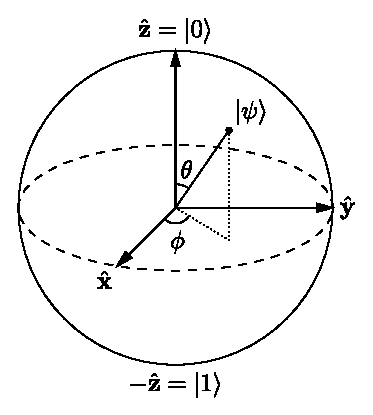
\includegraphics[scale=0.6]{bloch.eps}}
  \caption{Сфера Блоха як представлення квабіта $|\psi\rangle$}
\end{figure}
\end{definition}

\begin{definition} (Квантова система).
\end{definition}

\begin{definition} (Еволюція системи).
Темпоральна еволюція стану системи описується рівнянням Шрьодінгера:
$$
i\hbar\frac{\delta}{\delta t}|\psi\rangle = H|\psi\rangle.
$$
де $\hbar \equiv 1.05457 \cdot 10^{-43}$ експериментальна константа Планка,
а $H$ --- фіксований самоспряжений оператор на гільбертовому просторі,
знаний як Гамільтоніан квантової системи. В квантовій фізиці нормують відносно
$\hbar$ тоді рівняння можна записани у безвимірній формі $i|\psi\rangle = H|\psi\rangle$.
Гамільтоніан H повністю визначає квантову систему.
Другий спосіб визначення, через унітарний оператор $U=e^{-iH}$.
Темпоральна еволюція замкненої квантової системи зі страну $|\psi\rangle$ та часу $t_1$
в стан $|\psi'\rangle$ та часу $t_2$ може бути описана унітарним оператором
$U = U (t_2 - t_1)$, таким, що $|\psi'\rangle = U |\psi\rangle$.
\end{definition}

\begin{definition} (Вимірювання).
Проективне вимірювання визначається як самоспряжений оператор M який називається
спостереженням зі спектральною композицією $M = \Sigma_m mP_m$, де $P_m$ проекція
на власний простір власного значення m. Власні значення m оператора M відповідаються
усім можливим результатам вимірювання. Вимірювання $|\psi\rangle$ дасть результат
m з вірогідністю $p(m) = \langle\psi|P_m|\psi\rangle$, таким чином через
скорочення $|\psi\rangle$ отримаємо новий стан системи $|\psi'\rangle = \frac{1}{\sqrt{p(m)}}P_m|\psi\rangle$.
Для стану квабіта, самоспряжений оператор N знаний як стандартне вимірювання.
$$
N = \begin{pmatrix} 0 & 0 \\ 0 & 1 \end{pmatrix} = 0 \cdot |0\rangle\langle 0| + 1 \cdot|1\rangle\langle1|.
$$
Біль загально для простору стану $H=C^n$ стандартне вимірювання визначається як $N=\Sigma_i i|i\rangle\langle i|$.
\end{definition}

\begin{definition} (Виважене середнє).
Виважене середнє $\langle M \rangle$ усіх можливих результатів вимірювання M називється
очікуваним значенням та визначається як
$$
\langle M\rangle = \Sigma_n p(m)m = \Sigma_m \langle\psi|m P_m|\psi\rangle = \langle \psi | M | \psi \rangle.
$$
\end{definition}



\section{Огляд існуючих мов}

\subsection{Імперативні мови програмування}

\subsection{Квантові лямбда числення}
Загалом з огляду таксономії лямбла числень, яку виконав Хенк Барендрегт та подав
у вигляді лямбда кубу, можна розширити квантовими мовними примітивами будь яке
лямбда-числення (яке належить до лямбда кубу) або навіть вводити в
вищі лямбда числення з гомотопічними типами та
в системи доведення теорем з екстрактом або лише типизацією та обчисленнями на рівні типів.

\begin{definition} (Синтаксичне дерево $O_H$).
Синтаксичне дерево $O_H$ визначає лямбда числення з лінійними змінними
поєднане з класичним нетипизованим лямбда численням. Тобто $O_H$ є
найпростішим операційним квантовим лямбда численням для середовищ виконання.
\begin{lstlisting}[mathescape=true]
t = x
  | $\lambda$ x . t
  | t t
  | t
  | c
  | ! t
  | $\lambda$ ! x . t

c = 0 | 1 | H | S | $R_3$ | CNot | X | Y | Z | ...
\end{lstlisting}
Тут даються примітиви лінійних типів, де доступ до змінної
можливий лише раз в обсласті визначення змінної. Для нелінійних або звичайних
лямбда функції даються примітиви позначені !. В переліку квантових примітивів
c даються:
i) ортонормований базис $|0\rangle$ та $|1\rangle$;
ii) H --- оператор Адамара;
iii) S --- фазовий вентиль;
iv) $R_3$ --- $\pi/8$ вентиль;
v) контрольований не вентиль CNot;
vi) вентилі Паулі X, Y та Z.
\end{definition}

\section{Висновки}

\bibliographystyle{plain}
\bibliography{quantum}

\end{document}

